\chapter{Experiments 01}
\label{chapterlabel}


% Evaluation method and calibration 
% Detector Cal 
% System Cal 
% System evaluation 
% hard ware issues 

% New Event Recon (killed_LRF, FilteredSpectrum, Normalisation)
% New Linearity software (3 methods) 
In this chapter the use of the \acrshort{INSERT} scanner is outlined. The calibration procedures and experimental methods explored in this chapter are used to evaluated the system performance. The outcome of this investigation results in the implementation of new data processing methods. 

\section{Introduction}
The following experiments were carried out at San Raffaele Hospital (Milan), in collaboration with Politecnico di Milano (POLIMI). The system was transported and installed in the nuclear medicine department in order to carry out experiments with radioisotopes such as Technetium-99m. The experiments were carried out using the BULMA software provided by Mediso Ltd (Budapest). The software was designed to operate the system and acquired the raw data from experiments. The raw data was processed and calibrated using the BULMA INSERT-GUI package along with existing system data. 

This experiments set out to acquire the first phantom images from the \acrshort{INSERT} system, in order to achieve this the system was first evaluated and calibrated. The count-rate and energy resolution were determined and the system corrections and calibrations for these parameters where carried out at Polimi. The calibration procedures required to correct for event and image reconstruction are outlined here.

The calibration procedure was developed on a single detector head system \cite{DebCal}, and was tested in this investigation for the first time on the complete \acrshort{INSERT} scanner. This investigation aimed to determine the effectiveness of the proposed calibration method, and evaluate the systems performance and imaging capabilities. The calibration involves two stages, the detector calibration and the system calibration. The event reconstruction was corrected through the detector calibration procedure; a standard linearity and uniformity correction was performed. The image reconstruction was carried out using the geometric and sensitivity information obtained by the system calibration.

%\section{Methods}
\section{Detector Calibration}
The detector calibration is carried out by collecting uniformity and linearity data from each detector head. The uniformity of a given detector head is determined by the intensity variation across a planar acquisition. The uniformity is subject to spatial variations in the crystal properties such as, stopping power and number of emitted scintillation photons. Linearity is a measure of location dependent spatial distortion. This measured by reproducing a known linear geometry. Both uniformity and linearity are subject to position and time variations and so we must calibrate each detector regularly.

The uniformity data is collected by performing a flood scan of a single point source (1 MBq of $^{99m}Tc$) located in the centre of the scanner\acrshort{FOV}. The uniformity scan was carried out without the collimator attached; consequently short scans are required due to the high counts. The uniformity scans were collected once and used to correct for uniformity in the subsequent phantom acquisitions. 

The linearity distortion in a given detector was measured by acquiring data from a planar phantom (4 MBq of $^{99m}Tc$) mounted a set of parallel line collimators. Two collimator scans are carried out on each head; measuring the distortion in the X and Y direction respectively. The phantom attached of linearity collimator covered the whole detector head and so each unit was scanned individually. 40, 4 minute scans were required to collect the complete set of X and Y linearity data. 

\subsection{Detector Calibration Software}
The resulting data is processed using the BULMA software. The uniformity and linearity data is used to produce a set of transformation maps which are applied during the planar event reconstruction. As discussed previously the planar event reconstruction is carried out in a two step method; a centroid reconstruction is used to initialise an \acrshort{ML} reconstruction. Part of the \acrshort{ML} algorithm is the modelling of the detectors spatial response, the aforementioned \acrshort{LRF}. The BULMA software included existing \acrshort{LRF} data for the system, however it was found that this data was incorrect for the current system. The uniformity flood was used to produce a new set of \acrshort{LRF} models, which were incorporated in the event reconstruction.

The \acrshort{LRF}, uniformity, and the X/Y linearity data are input into the BULMA software alongside the raw uncorrected phantom data. The X and Y data are firstly reconstructed to produce two planar images of linear bands. The software uses active contour splines to identify the data bands. The resulting X and Y splines are combined to produce a grid of crossing control points; the linearity map is created. The photopeak of the total phantom data is determined and an initial reconstruction is found using the \acrshort{LRF}. The linearity map crossing points mark out positions to determine the local energy spectra; these produce a local, position-dependent, energy filter. The energy at each pixel position in the phantom reconstruction are calculated and matched to the local energy map. Correcting for the local energy peaks produces a planar reconstruction corrected for energy and linearity. The uniformity data is reconstructed in the same way to create the uniformity map. The phantom reconstruction is multiplied by the inverse of the uniformity map to correct each pixel. The final result is corrected planar image, ready for image reconstruction. 

%\subsection{Uniformity}
%\subsection{Linearity} 

\section{System Calibration}
The image reconstruction algorithm requires information of the systems geometry and sensitivity. The system calibration acquires this information through two experiments. Each experiment is carried out with the collimator fitted. The data from each experiment produces correction which are applied to the planar images during image reconstruction. 
 
The geometric calibration has been established previously, \cite{8340862}. The geometric data is acquired from a series of scans of capillary phantoms. The capillaries have 1 mm diameter and are filled with 10 MBq of $^{99m}Tc$. Two experiments are set up to acquire the axial and trans-axial geometry of the system. 

\textbf{Axial Orientation:} The capillaries were aligned with the axial direction of the scanner. The capillaries are held on a rotating stage and positioned at 4 locations with the \acrshort{FOv}. The positions are separated by 90\degree and lie at radii of 25, 50, 75 and 100 mm. From these positions the capillaries are rotated about the z axes of the scanner. The capillaries are scanned for 2 minutes at 30 positions; rotating by 12\degree until 360\degree is covered. 

\textbf{Trans-axial Orientation:} similarly the capillaries were placed along the trans-axial plane and rotated about the z axes. Five capillaries are at positions, 0, \pm 5, \pm 10 cm from the centre of the bore. Due to time constraints these capillaries were only scanned for 5 positions.

The sensitivity calibration required data with a planar phantom, $10 * 10 * 0.5$ cm, filled with 50 MBq of $^{99m}Tc$. The phantom was place in front of each detector head and scanned individually. The phantom covered the whole collimator \acrshort{FOV}, the resulting flood acquisition gave a measure of uniformity variation due to the collimator geometry. 

\subsection{System Calibration Software}
The data collected from the system calibration undergoes planar event reconstruction and detector calibration as described above. The resulting data was analysed in MATLAB.

The geometric data was used to measure 3 system parameters of the collimator. The tilt and twist angles, and mechanical shifts were determined by modelling the variation in position and size of the capillary data. The location of each capillaries is measures with a Gaussian model by taking measurements along its length. The variation in position as a function of radial position of the axial capillaries is known as the mechanical shift in the collimator. The variation of position along the length of a trans-axial capillary is known as the twist angle. Finally the variation in position as a function of radial position of the trans-axial capillaries gives us a measure of the tilt angle.

The reconstructed sensitivity profiles gave a measure of count variation across the whole collimation. The sensitivity variation as a function of sampling angle of the aperture was modelled. Each profile was fitted using equation (\ref{sens_model}), where $\phi$ is the sampling angle, $G_{\sigma}(\phi)$ is a Gaussian function and the summation is done over all mini-slits $i$ for each collimator section $j$. 

\begin{equation}
%\vspace{-0.2cm}
\label{sens_model}
S_{j}(\phi) = \sum_{i} G_{\sigma}(\phi) \ast A_{i,j} \cos^{p}{\phi} + b_{j}(\phi)
%\vspace{-0.2cm}
\end{equation}

The final step in the calibration involves re-sampling the projection data to produce projection reconstructions in object domain. Accounting for the system geometry, the radial position of each event is calculated. The events are then re-ordered with respect to the radial position from the centre of the FOV. The result allows for easier visual analysis of the acquired data; at this stage the data are completely corrected and ready for reconstruction. 

\begin{figure}[!t]
%\vspace{-0.2cm}
\centering
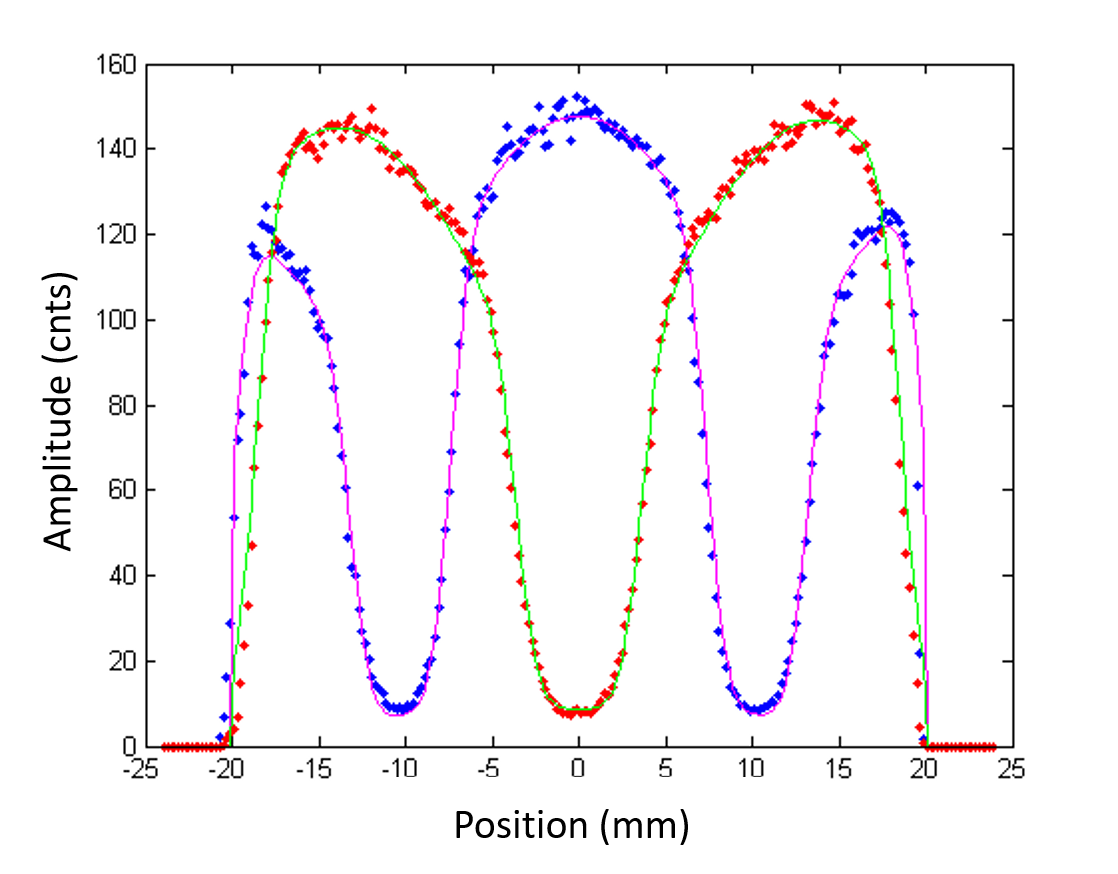
\includegraphics[width=2.9in]{figures/sns_prof.png}

\caption{Sensitivity profiles for two collimator sections and fitted analytical functions.}
\label{fig_sensprof}
%\vspace{-0.2cm}
\end{figure}

\subsection{System Calibration}
\subsection{Geometry}
\subsection{Sensitivity}

As can be expected from the initial testing of a prototype
the system had issues with both hardware and software during
this research. We have been able to identify these issue,
implement corrections to overcome them and plan for future
improvements to the system and our experimental method. The
hardware issues reside in an instability in the detector modules.
Each SiPM readout is comprised of 72 channels, of which 2
of the total 1,440 produced the incorrect signal and had to be
switched off during most acquisitions. To correct this we were
able to amend the Mediso software and produce a correction
algorithm which was able to interpolate the missing data. This
provided a powerful means of producing projections despite
missing data. In future a more stable solution would be to
replace the readouts. This example demonstrates the kind of
issues encountered in this work; due to inexperience with a
novel system, requiring retrospective software solutions, and
solved in future with final hardware solution.
The final tomographic images were subject to a number
of corrections and post processing, some were inherit to the
system design where others were subject to our experimental
method. Despite this, we were able to extract the desired
images parameters and produce a set of phantom acquisitions
as a proof of concept.

\section{Methods}
Here we discuss the methods used to acquire the relevant
data and apply it to our image reconstruction procedure.
The image reconstruction algorithm follows a standard
Maximum Likelihood Estimation Maximisation (MLEM) algorithm,
however, the INSERT system requires the aforementioned
system corrections and resolution modelling to account for the MSS geometry. The following sections outline
the methods required for image reconstruction and how we
adapted them for the complete 20 detector system.

\subsection{Initial System Testing}
\subsection{Count-rate} 
\subsection{Energy}
\subsection{Resolution}
\subsection{Detector Calibration}
\subsection{Uniformity}


\subsection{Linearity} 
\subsection{System Calibration}
\subsection{Geometry}
The geometric calibration procedure was required to account
for the MSS geometry. The full ring procedure was not
changed from the previous design, [2]. The MSS collimator
is installed and a set of vertical and horizontal capillaries
are scanned. The acquisitions from set of capillary sources
are corrected for linearity and uniformity with the previous
procedures. The resulting images were used to determine
a set of Twist and Tilt parameters required in the image
reconstruction. The Twist and Tilt parameters determined the
angles of distortion in the axial direction and trans-axial
plane respectively. The angles were calculated by a measure
of relative position of the capillary sources and modelling
the distance as a function of the radial position. Extracting
these parameters allowed us to correct the distortion in the
projections caused by the collimator geometry.
The capillary sources served a second purpose; by combining
the acquisitions we produced an image of 61 capillary
sources spanning 5 radial positions. This image was used to
determine the image resolution of the system subject to radial
position. By modelling the capillaries in a the trans-axial plane
with a 2D Gaussian, we determined the radial and tangential
image resolutions.

\subsection{Sensitivity}
\subsection{Phantom Acquisitions}
\subsection{Capillary}
\subsection{Cylinder}
\subsection{Cold Rods}
\subsection{Hot Spheres} 
\subsection{Hoffman}

\section{Results}
%\subsection{Initial System Testing}
%\subsection{Count-rate} 
%\subsection{Energy}
%\subsection{Resolution}
\subsection{Detector Calibration}
Initial testing of the system performance revealed the presence of faulty channels in some detector head. A faulty channel would produce a high number of false counts which resulted in a hot spot; drowning out the healthy channels and giving counts to neighbouring pixels. The solution to this was to turn off the offending channels and leave a single dead pixel in its place. The dead channel left a large gap in the projection data; event reconstruction was carried out but detector calibration was not possible. The \acrshort{LRF} provided a solution to this problem as it gave the spatial response for each individual channel. The killed channels were therefore modelled as a such in the \acrshort{LRF} data. This allowed the \acrshort{MLEM} reconstruction to model the missing data and interpolate events from neighbouring channels. The modified reconstruction significantly reduced the data gap left by the faulty channel. 

\subsection{Uniformity}
\subsection{Linearity} 
\subsection{System Calibration}
\subsection{Geometry}
\subsection{Sensitivity}
Fig. \ref{fig_sensprof} shows examples of sensitivity profiles for two different collimator sections and the corresponding fits.
\subsection{Phantom Acquisitions}
\subsection{Capillary}
\subsection{Cylinder}
\subsection{Cold Rods}
\subsection{Hot Spheres} 
\subsection{Hoffman}

\section{Discussion}

\section{Conclusion}